
The quench simulation of the skew quadrupole is divided into two parts: $(i)$ analysis before the quench detection when the~current is constant, $(ii)$ analysis after the quench detection when the~current starts varying in time until the energy stored in the magnetic field is fully discharged. This section covers the simulation of the first case. 

\subsection{Mesh and Geometry}

Fig.~\ref{fig:skew_quad_ansys_top_view} shows the top view of a meshed ANSYS geometry. It consists of 754 insulated windings. In total, the coils is nearly~810 m-long. It is shorter than 812~m corresponding to the real magnet length because of sharp edges of the rounded coil parts. 

\begin{figure}[H]
    \centering
    \begin{tikzpicture} [scale=0.8]
    \node[scale=0.8] at (0,0) {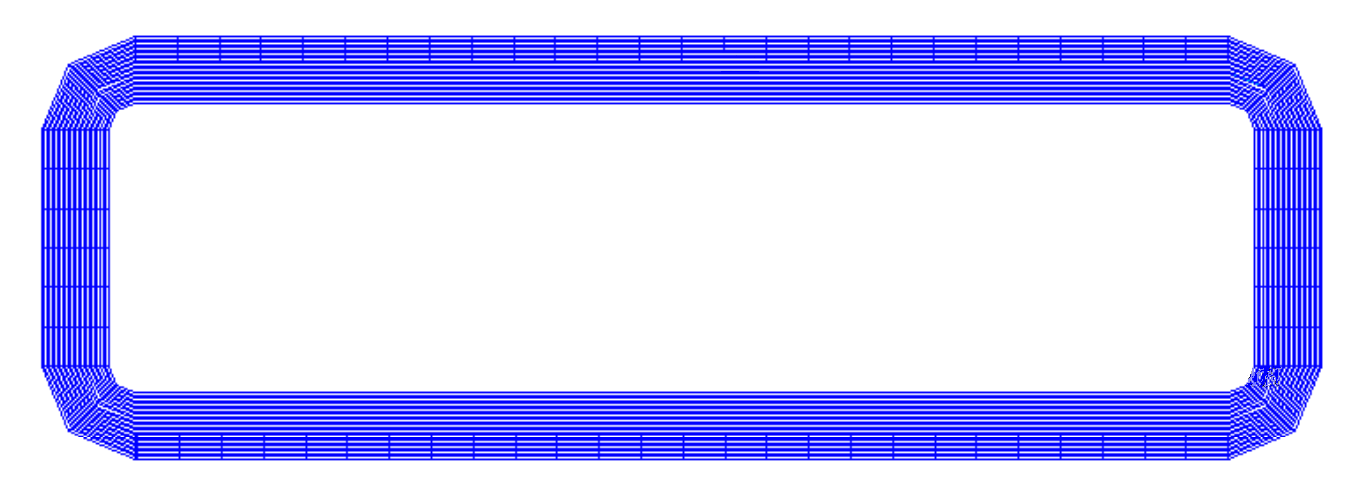
\includegraphics[width=.7\textwidth]{sections/skew_quad_q_det/figures/skew_quad_analysis/coil_top_view.png}};
    \end{tikzpicture}
    \caption{ANSYS meshed geometry of the skew quadrupole - top view.}
    \label{fig:skew_quad_ansys_top_view}
\end{figure}

Parameters of the meshed geometry are summarised in Table~\ref{table: skew_quad_geometry_mesh}. They are based on the discussion in Section~\ref{subsection:update_skew_quadrupole_geometry}. The insulation domain transverse to the strand is equal to $L_\text{ins}=0.07~\text{mm}$ that corresponds to the thickness of a real insulation layer (of only one strand) without resin. The insulation conduction area $A_\text{ins, cond}$ remains unchanged in this set of analyses, i.e. $u_\text{ins}=1.0$. The geometry is discretised on each side of the coil to uniformly distribute the the insulation conduction area $A_\text{ins, cond}$ along the entire domain of the windings. The parameter $n_\text{divisions, insulation}$ corresponds to an average length of a coil rounding. The parameters $n_\text{divisions, side d}$ and $n_\text{divisions, side e}$ refer to Fig.~\ref{fig: winding_length_in_skew_quad}.

There are 72 nodes in each winding representing the composite strand. The insulation layer of every winding is reduced to two elements. It means that the insulation layer between two neighbouring windings accounts for four elements out of which two are coupled with one another. Therefore, the insulation modelling sustains a basic condition of simulating non-linear phenomena that require using at minimum three nodes. The longitudinal mesh size is equal to 15~mm whereas the insulation mesh size -- 35~$\upmu \text{m}$. The entire discretised model accounts for approximately half a million of nodes. Reducing the number of insulation elements aims at lowering the total model size.

\begin{table}[H]
    \caption{Geometry and mesh characteristics.} 
    \vspace{-1.em} 
    \fontsize{10}{10}
    \selectfont 
    \renewcommand{\arraystretch}{1.5}
    \begin{center}
        \begin{tabular}{ ccc }  
        \hline
        parameter & value & unit \\
        \hline
        $L_\text{coil, ANSYS}$ & 809.9 & [m] \\
        $L_\text{ins}$ & 0.07 & [mm] \\
        $A_\text{ins, cond}$ & $8.75 \cdot 10^{-6}$ & [$\text{m}^2$] \\
        $u_\text{ins}$ & 1.0 & [-] \\
        $n_\text{divisions, insulation}$ & 2 & [-] \\
        $n_\text{divisions, winding}$ & 64 & [-] \\
        $n_\text{divisions, side d}$ & 26 & [-] \\
        $n_\text{divisions, side e}$ & 6 & [-] \\
        mesh size, insulation & 35 & [$\upmu \text{m}$] \\
        average mesh size, strand & 15 & [mm] \\ 
        nodes in coil & 478 000 & [-] \\
        \hline 
        \end{tabular}
    \end{center}  
     \label{table: skew_quad_geometry_mesh} 
 \end{table}

There are three quench analyses conducted with a varying heat capacity of resin that refers to the parameter $u_\text{resin}$, as depicted in Table~\ref{table: skew_quad_geometry_cases}. Adding 0D elements to the strand increases the total number of elements in the model from 480 000 to 530 000. 

\begin{table}[H]
    \caption{Geometry and mesh characteristics.} 
    \vspace{-1.em} 
    \fontsize{10}{10}
    \selectfont 
    \renewcommand{\arraystretch}{1.5}
    \begin{center}
        \begin{tabular}{ c | c | c }  
        \hline
        $u_\text{resin}$ & $V_\text{MASS71}$, [$\text{m}^3$] & elements in coil \\
        \hline
        0.0 & 0.0 & 476 528 \\
        0.5 & $2.4 \cdot 10^{-9}$ & 531 574 \\
        1.0 & $4.8 \cdot 10^{-9}$ & 531 574 \\
        \hline 
        \end{tabular}
    \end{center}  
     \label{table: skew_quad_geometry_cases} 
 \end{table}

\subsection{Analysis Settings}

The co-simulation time window remains identical with respect to the previous chapters, as depicted in Table~\ref{table: skew_quad_quench_detect_input_params}. The ANSYS simulation time step is assumed to be constant and equal to the maximum value of a time step range used for the quench velocity-based approach in Chapter~\ref{chapter:quench_velocity_benchmarking}. The time step is increased to keep the computing time in a reasonable limit of several days. The initial energy deposition is placed in the centre of a winding directly neighbouring with the spot heater corresponding to the position of 367.67~m in the meshed model.

\begin{table}[H]
    \caption{Input parameters in the quench detection analysis of the skew quadrupole.} 
    \vspace{-1.em} 
    \fontsize{10}{10}
    \selectfont 
    \renewcommand{\arraystretch}{1.5}
    \begin{center}
        \begin{tabular}{ ccc }  
        \hline
        parameter & value & unit \\
        \hline
        $t_\text{com}$ & 2.5 & [ms] \\
        $t_\text{step}$ & 1 & [ms] \\ 
        hot-spot position in coil & 367.97 & [m] \\
        \hline 
        \end{tabular}
    \end{center}  
     \label{table: skew_quad_quench_detect_input_params} 
 \end{table}

\subsection{Results}

The evolution of resistive voltage until the quench detection is shown in Fig.~\ref{fig: quench_detection_v_res}. The results from three analyses are compared with the measurements. One can observe that the~initial slope of the~simulated models and the measured magnet remains similar at $t < 0.1~\text{s}$. It means that the~initial quench velocity set in the model corresponds to its real value in the quenched winding at $I=86~\text{A}$. In the measurements, the first turn-to-turn propagation occurs at $t \approx 0.08~\text{s}$ which is much faster than in case of each simulation. However, one must remember that the initial heat impulse is much larger in the measurements than in the simulated cases. Therefore, the~first transverse propagation also occurs more slowly in the simulations compared to the measurements. Including resin in the models results in a slower turn-to-turn propagation as well. Such a phenomenon is expected due to a higher heat capacity of the windings with resin. 

\begin{figure}[H]
    \centering
    \begin{tikzpicture}
        \begin{axis}[
          no markers,
          width=0.7\linewidth, 
          height = 4.0cm,
          xlabel={$t,~\text{s}$},
          ylabel={$V_\text{res},~\text{V}$},
          xmin=0.0,
          xmax=0.5,
          xtick= {0,0.1,0.2,0.3,0.4,0.5},
          ymin=0.0,
          ymax=0.5,
          legend pos = outer north east
          ]
          
          \addplot[green] table[x=time,y=V_res,col sep=comma] {sections/skew_quad_q_det/figures/skew_quad_analysis/results_case1.csv}; 
          
          \addplot[blue] table[x=time,y=V_res,col sep=comma] {sections/skew_quad_q_det/figures/skew_quad_analysis/results_case2.csv}; 
          
          \addplot[red] table[x=time,y=V_res,col sep=comma] {sections/skew_quad_q_det/figures/skew_quad_analysis/results_case3.csv}; 
          
          \addplot[black, dashed] table[x=time,y=V_res,col sep=comma] {sections/skew_quad_q_det/figures/skew_quad_analysis/measurements.csv}; 
          
          \addplot[black, dotted] table[x=time,y=QDS_v_threshold,col sep=comma] {sections/skew_quad_q_det/figures/skew_quad_analysis/measurements.csv}; 
          
          \legend{
          $u_\text{resin}=0.0$,
          $u_\text{resin}=0.5$,
          $u_\text{resin}=1.0$,
          measurements}
          
        \end{axis}
    \end{tikzpicture}
    \caption{Rise of resistive voltage.}
    \label{fig: quench_detection_v_res}
\end{figure}

Once the first turn-to-turn propagation occurs, the simulated models start resembling the measurements because the current discharged in the coil becomes a predominant heat source. In order to compare the measurements with the performed analyses, each resistive voltage obtained in the simulations is translated to the left so that the~threshold voltage $V_\text{th}$ is reached at the same time window. Table~\ref{table: skew_quad_v_res_q_det} presents the~time windows at which the~threshold voltage is obtained for every case. The translation times are used in the next section to translate the plots of the resistive  voltage and resistance from the simulations. By that means, the comparison of the simulations with the results is more clear. 

\begin{table}[H]
    \caption{List of time windows at which the simulations reaches $V_\text{th}$.} 
    \vspace{-1.em} 
    \fontsize{10}{10}
    \selectfont 
    \renewcommand{\arraystretch}{1.5}
    \begin{center}
        \begin{tabular}{ cccc }  
        \hline
        parameter & $t(V_\text{th})$ & $t_\text{translation}$ & unit \\
        \hline
        measurements & 0.13 & - & [s] \\
        $u_\text{resin}=0$ & 0.30 & -0.17 & [s] \\
        $u_\text{resin}=0.5$ & 0.36 & -0.23 & [s] \\
        $u_\text{resin}=1.0$ & 0.40 & -0.27 & [s] \\
        \hline 
        \end{tabular}
    \end{center}  
     \label{table: skew_quad_v_res_q_det} 
 \end{table}